\chapter{Narrativa visual: a pintura brasileira de Lucia Laguna e Cristina Canale}\label{cap3-narrativa-visual}

As referências de outros pintores nos fornecem pistas, mas um objetivo
comum a muitos artistas é encontrar o seu próprio modo de construir
narrativas. Queremos saber como os pintores alcançam um resultado
satisfatório para si mesmos, em seus projetos, trazendo referências
pessoais e externas, para seu processo criativo. Partimos de nossa
trajetória nos estudos do cinema e da pintura, aprofundada nas
experimentações plásticas do mestrado. Entretanto, tornou-se necessário
investigar como outros pintores estabeleceram seu repertório de
referência para desenvolver suas poéticas. Recorremos, neste capítulo,
à obra de duas artistas brasileiras, Lucia Laguna (1941) e Cristina
Canale (1961), cujo processo encontra pontos de contato com reflexões
presentes nesta dissertação. Analisamos, então, o desenvolvimento dos
projetos artísticos destas duas pintoras, no que diz respeito à forma
como trazem referências estéticas internacionais e atemporais para seus
trabalhos e as mesclam com sua própria cultura
visual.\footnote{\fullcite{medeiros2017cultura}. Em 1924, o teórico do
	cinema Béla Balázs em um dos seus textos de \emph{O Homem visível}
	(\emph{Der Sichtbare Mensch}) sugere que a invenção do cinema conduzirá
	a cultura conceptual da palavra em direção a uma \emph{cultura visual}
	\textins{\emph{visuelle Kultur}}. Na verdade, esta última teria sido
	dominante até à invenção da imprensa, o cinema ajudando \textquote{Balázs, 2017}{a humanidade
		inteira \textelp{} a aprender a linguagem desaprendida das mímicas e dos
		gestos}}

\section{Quem nasceu primeiro: o artista, a obra ou o observador?}%
\label{sec:quem-nasceu-primeiro-o-artista-a-obra-ou-o-observador}

Na coleta de material sobre as artistas Lucia Laguna e Cristina Canale,
para fins de análise de seus processos, nos apoiamos em três tópicos: o
artista, a obra em si e o observador ou crítico. Em um primeiro
momento, trazemos informações que encontramos em depoimentos destas
pintoras sobre seu processo. Estas declarações estão em forma de textos
escritos por si mesmas, como a autobiografia, \emph{statements} ou
declarações e nas entrevistas que concederam em vídeos e à mídia. A
importância do discurso do artista na primeira pessoa é destacada por
\textcite{ferreira2006escritos}
ao argumentar que a reflexão teórica, a
partir dos anos 60, é centrada nos problemas correntes da própria
produção. Segundo \textcite{ferreira2006escritos}, estes escritos podem ser remetidos ao
século~XV, à passagem do \emph{pintor} ao \emph{artista}, do
\emph{artesanato} às \emph{belas-artes}, revelando condições
socioculturais do artista e de sua personalidade.

Ao selecionar uma amostra de obras de diferentes períodos, buscamos
verificar como foi construída a narrativa visual do espaço pictórico,
ao longo de suas trajetórias, diante da investigação plástica e adoção
de métodos individualizados para a sua produção.

\newpage

A investigação no âmbito da arte contemporânea se funda, atualmente, em
um complexo sistema que vai além do texto acadêmico. Desta forma, além
do que dizem as próprias artistas, tomamos por base textos de outros
autores, tanto a nível curatorial de exposições realizadas por estas
pintoras, quanto textos críticos de revistas, que podem agregar outros
pontos de vista, para a compreensão da manifestação artística que
ocorre no ateliê.

\section{Lucia Laguna --- Paisagem urbana, geometria, colagem e Dadá}%
\label{sec:lucia-laguna-paisagem-urbana-geometria-colagem-e-daduxe1}

Lúcia Laguna é uma pintora, residente no Rio de Janeiro, nascida na
cidade de Campos dos Goitacazes. Em entrevista para a 30\textordfeminine.~Bienal de
São Paulo~(2012), a artista nos conta que o seu assunto é o espaço no
seu entorno, a paisagem a partir da janela, do bairro da Mangueira, o
próprio ateliê, com cadeiras, mesas e telas que se sobrepõem no espaço
reduzido, e o seu jardim. Para esta exposição, Lúcia organizou as 35
telas que preparou para atender o convite da Bienal, em diversos
formatos e tamanhos, sendo os maiores com dimensões de 3 metros de
largura e os menores com 15 cm. Segundo ela, o objetivo era montar os
trabalhos na sala desta exposição da mesma forma como estavam dispostos
em seu ateliê, sem a tradicional organização enfileirada de uma
galeria. Nesta entrevista, Lúcia já deixa claro que um de seus
processos inclui a pintura simultânea de quadros maiores e menores, com
a finalidade de aproveitar a tinta para estes últimos. Outro dado que
nos apresenta a artista ao falar sobre a alternância de obras na
exposição, durante o período da Bienal, é que seus quadros são pintados
já na tela, ou chassi, e que vai girando os trabalhos. Desta forma os
trabalhos finais apresentam várias faces. Estas estratégias podem
parecer simplistas, a princípio, mas sabemos o quanto a escolha das
dimensões e do formato pode ser decisiva para a resolução plástica de
uma imagem, assim como a experimentação de novas posições relacionadas
à verticalidade (Bienal de São Paulo,~2012).

Em uma entrevista anterior, para o vídeo de \textcite{cupello2007laguna},
Lucia apresenta a série de pinturas \emph{Entre a Linha Vermelha e
	Amarela}, e fala sobre suas inúmeras referências bem como a forma como
lida com elas. A paisagem do subúrbio que Lucia vê, através de sua
janela, é uma das bases de seu trabalho. Ela nos conta que via os
carros passando sobre esta estrada no Rio de Janeiro chamada Linha
Vermelha cuja estrutura de ferro chamou sua atenção. Assim surgiu o
título desta série, que cria um jogo de palavras entre o nome das
estradas cariocas e as cores presentes em sua pintura.

Além de plantas, Lucia cultiva referências visuais de muitos pintores e
lança mão delas quando folheia os muitos livros que mantém em seu
ateliê. Na parede escreve, em sequência, os nomes de todos aqueles que
carinhosamente chama de Família. O conceito de cultura visual está
presente na história da arte e significa o conjunto das atividades e
instituições relacionadas com a produção, criação e divulgação das
artes e ciências humanas.\footnote{\enquote{cultura}\textbf{,} in
	Dicionário Priberam da Língua
	Portuguesa,~\url{https://dicionario.priberam.org/cultura} (acesso
	em 5 de janeiro de 2022).} Do período renascentista à pop arte, temos muitos
exemplos de intercâmbios de pintores e artistas que viajavam entre
países e continentes, realizando a troca de suas \emph{bagagens
	culturais}. Uma das referências citadas no vídeo, por Lucia, é o pintor
\emph{Paolo Uccello} (1397--1495). \enquote{Este pintor italiano
	renascentista era obcecado pela perspectiva e passava noites tentando
	entender o Ponto de Fuga, que usava para criar uma sensação de
	profundidade em suas obras e não para narrar histórias.} Percebemos uma
identificação com este pintor, no traçado de linhas com a fita crepe
utilizada por Lúcia, ao representar a paisagem da janela, na série
\emph{Entre a Linha Vermelha e Amarela}.

\begin{figure}
	\begin{minipage}[b]{.45\linewidth}
		\caption{\artname{Lucia Laguna}{Entre a Linha Vermelha e a Linha Amarela n\textordmasculine.~14}{2003}}
		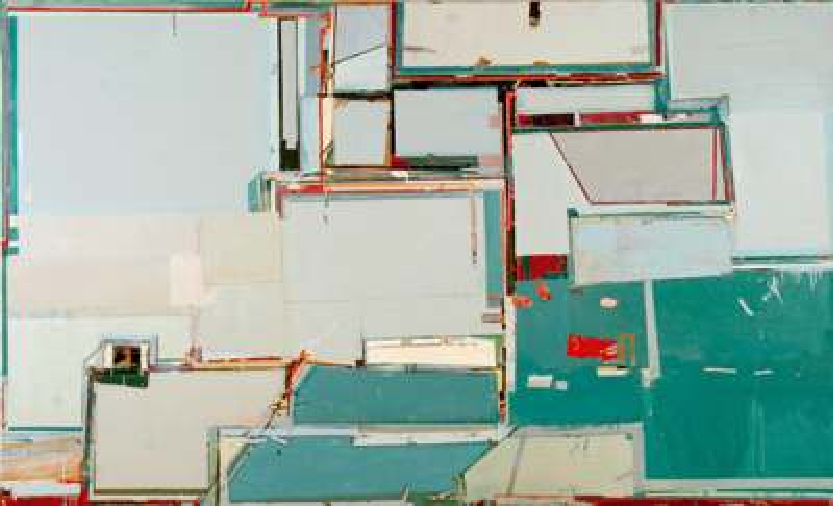
\includegraphics[width=2.2769in,height=1.96429in]{figuras/laguna-entre-linha-vermelha-linha-amarela14-2003.pdf.compressed.pdf}

		\figurenote{Registro fotográfico Amilcar Packer.
			Fonte: \hiperlink{enciclopedia.itaucultural.org.br/obra63784}{Enciclopédia Itaú Cultural}}
	\end{minipage}\hfill
	\begin{minipage}[b]{.45\linewidth}
		\caption{\artname{Lucia Laguna}{Entre a Linha Vermelha e a Linha Amarela n\textordmasculine.~44}{2005}}
		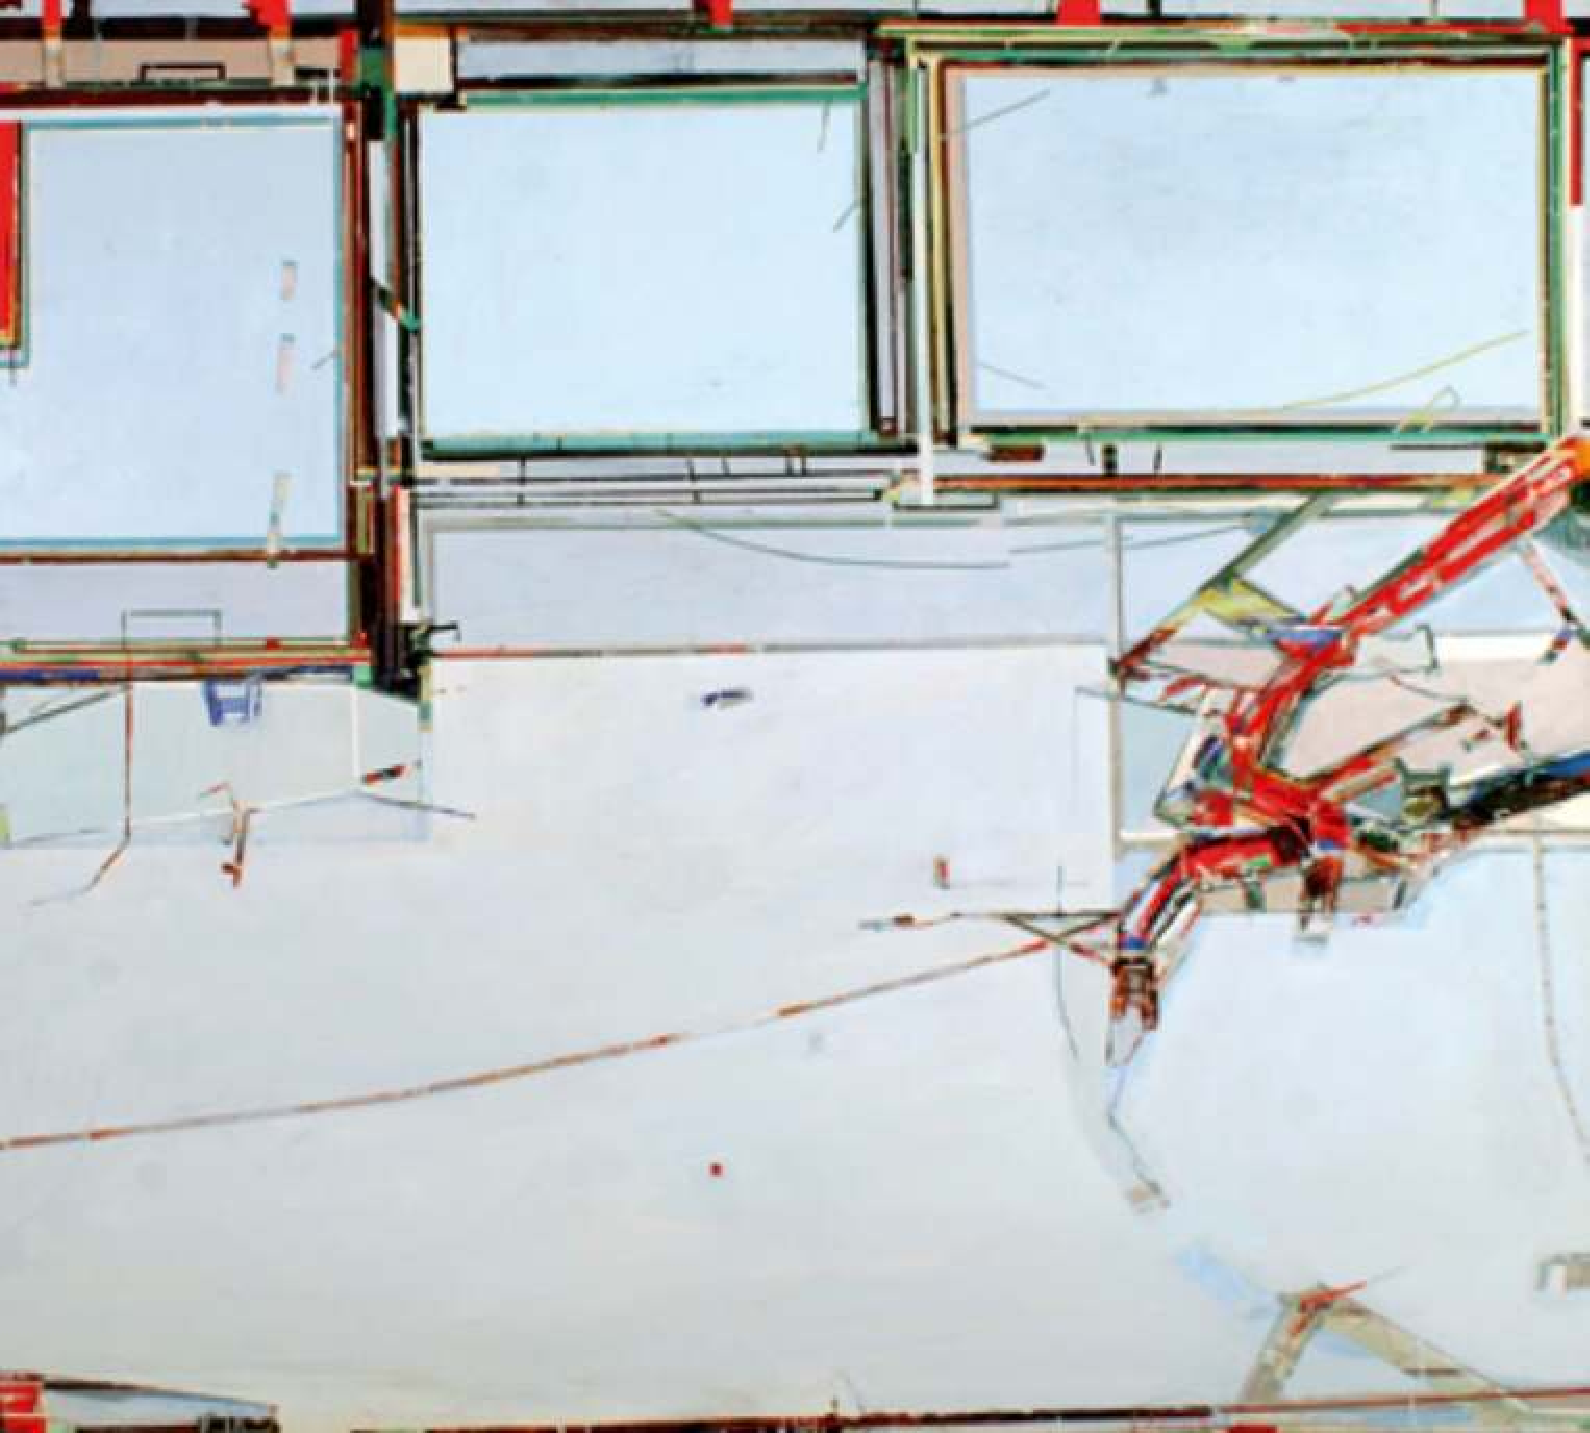
\includegraphics[width=2.16964in,height=1.95646in]{laguna-entre-linha-vermelha-linha-amarela44-2003.pdf.compressed.pdf}
		\figurenote{Reprodução Fotográfica Amilcar Packer. Fonte: \hiperlink{enciclopedia.itaucultural.org.br/obra63784}{Enciclopédia Itaú Cultural}}
	\end{minipage}
\end{figure}

No entanto, um certo mistério permanece no ar, como traduz bem o
professor \textcite{couto2021lucia}:

\begin{displaycquote}{couto2021lucia}[.]
	Sabemos que as pinturas retratam a paisagem do Morro da Mangueira que
	ela vê de seu ateliê, assim como as vias expressas da Linha Amarela e da
	Linha Vermelha. Porém, não conseguimos identificar os símbolos dessas
	paisagens marcantes da cidade. Se ela codifica esses pontos, por que
	então não os reconhecemos? Nos termos de Koselleck (1923--2006), o
	\emph{espaço de experiência} da artista, o corpo atravessando esses
	lugares e o olhar decodificando essas marcas já são embebidos por outras
	substâncias que atuam em seu processo técnico. É por isso que vemos
	longas retas que atravessam e dirigem territórios pictóricos espessos
\end{displaycquote}

É preciso lembrar que as referências nem sempre se traduzem no trabalho
de forma muito clara. O interesse por Paolo Uccello e a
movimentação provocada no olhar do espectador pelas espadas da
\emph{Batalha de São Romano} não se transmutam em uma figuração fácil em
Laguna. Porém, Lucia testa nosso~olhar fazendo-o percorrer planos e
linhas que muitas vezes se interrompem, mantendo assim~nosso interesse
em decifrar o seu código.

Entre pintores vivos e antepassados, que conheceu nos livros e nas
viagens para museus proporcionadas pelos cursos do Parque Lage com
Charles Watson, Lucia relaciona influências abstrato/figurativas como a
do pintor Richard Diebenkorn, e explica o processo das sobreposições de
fita crepe e tinta a óleo para manter seções do trabalho. Neste
processo a surpresa quando retira a fita crepe é um dos fatores que
julga mais interessantes. Declara, ainda, que criou um processo, nesta
série \emph{Entre a Linha Vermelha e Amarela}, para tentar esconder a
pintura gestual, que tanto aprecia, como a de Willem de Kooning, e que
por volta do ano de 1994, quando começou a pintar, era um tipo de
pintura \enquote{execrada} no meio da arte contemporânea.

Embora tenha características narrativas muito fortes, a pintura de
Paula Rego (1935--2022) é vista por Lucia Laguna como um exemplo de quem
faz algo que se parece com o que ela faz: a colagem \parencite{cupello2007laguna}. Em
outras palavras, o processo de colagem tem uma relação muito importante
com o seu trabalho.

É importante lembrar que, a colagem é um procedimento técnico que tem
origem muito antiga, e que acompanha movimentos artísticos da vanguarda
que surgem antes e depois da primeira guerra mundial, como o Cubismo, o
Dadaísmo, o Futurismo e o Surrealismo.

\begin{displaycquote}{enciclopedia2015colagem}[.]
	\textelp{} sua incorporação na arte do século XX, com o cubismo, representa
	um ponto de inflexão na medida em que liberta o artista do jugo da
	superfície. Ao abrigar no espaço do quadro elementos retirados da
	realidade --- pedaços de jornal e papéis de todo tipo, tecido, madeira,
	objeto e outro \textelp{}
\end{displaycquote}

Estes movimentos artísticos se apropriaram do cinema no início do
século XX.

\begin{displaycquote}[108]{ruzza2016dadaismo}[.]
	No campo da pintura, Duchamp é conhecido por duas obras famosas. A
	primeira é \emph{Nu descendant un escalier}\footnote{%
		Sobre Nu descendo as escadas, video \enquote{As escolhas dos críticos:
			Marcel Duchamp por Delfim Sardo \textbar{} Museu Coleção Berardo.}
		\url{https://youtu.be/-raCSeutwoI}}, se baseia na decomposição do
	movimento. Na tela, o artista apresenta uma sobreposição de figuras
	humanas, ou parecidas com seres humanos, descendo uma escada, sugerindo
	a ideia de um movimento contínuo, uma violação da concepção tradicional
	da imagem. Este trabalho de 1912 lhe valeu a ruptura com o movimento
	cubista, que o acusou de apresentar elementos futuristas, por causa das
	ideias de movimento, desintegração do espaço, maquinismo
\end{displaycquote}

Como já descrito no \cref{cap1-contexto-relacao-cinema-pintura}, a colagem
na pintura, guarda, em
diversos momentos históricos, interligações com o cinema. Influências
de ambas as partes, tanto por artistas e teóricos que se aventuram na
arte cinematográfica quanto em movimentos artísticos, com destaque para
o Futurismo e o Dadaísmo, este último interrelacionado ao cinema
expressionista alemão. Encontramos na palavra \emph{Colagem} o elo com
um momento da arte que nos interessa tratar, do movimento Dada, que
parece apropriado para pensar muitos dos processos e técnicas da
pintura contemporânea.

\begin{displaycquote}{enciclopedia2015colagem}[.]
	Diverso é o resultado da técnica no interior do movimento Dada. Em
	Marcel Duchamp (1887--1968) e Francis Picabia (1879--1953), nota-se uma
	radicalização dos procedimentos usuais da colagem, numa clara recusa ao
	que eles consideram a rigidez cubista. Nos trabalhos de Kurt
	Schwitters,\footnote{Sobre \emph{Kurt Schwitters}
		\url{https://www.youtube.com/watch?v=7GEIUvaEwrI\&ab\_channel=Sotheby\%27s}}
	(1887--1948) a ênfase recai sobre elementos e materiais diversos, que
	encontram seu exemplo mais acabado nas obras \emph{Merz} (1919). \enquote{A
		pintura Merz}, diz ele, \enquote{não utiliza só a cor e a tela, o pincel e a
		paleta, senão todos os materiais percebidos pelos olhos e todas as
		ferramentas necessárias.} \textelp{} Diferente é a trajetória seguida
	pelos artistas ligados à Bauhaus quando empregam a colagem e a montagem
	como parte de seu programa pedagógico. Distinto também o sentido que
	Henri Matisse (1869--1954) atribui aos papéis colados que utiliza na obra
	de maturidade, em que a pesquisa da forma liga-se diretamente à
	exploração da cor
\end{displaycquote}

Retomamos a análise da obra de Lucia Laguna, em um momento mais
recente, através da exposição \emph{Se ace caminho al andar,} realizada
em 2021, na Carpintaria, no Rio de Janeiro, \parencite{gabriel2022laguna},
onde a geometria das vistas da janela dá lugar a uma profusão de formas
e cores na representação do seu jardim. Nesta exposição, Lucia reforça
um dado fundamental do processo que desenvolveu através do trabalho
colaborativo com outros pintores no seu ateliê. Seu ponto de partida é
sempre uma proposição que faz aos assistentes, que inserem linhas,
figurações e outros sinais gráficos na tela. Ao assumir a execução da
obra, ela ingressa em um processo de desconstrução do que já estava
ali. Novos cenários são construídos em uma sucessão de camadas e
detalhes, onde sua preocupação é de manter parte do que já existia.
Para ela, tudo é
acúmulo.\footnote{\url{https://www.artequeacontece.com.br/lucia-laguna-revela-pinturas-feitas-durante-o-isolamento-social/}}

Passamos agora ao que dizem alguns críticos e curadores, atuantes no
cenário das artes brasileiras, sobre o processo criativo de Lucia
Laguna. Para o curador Marcelo Campos, \parencite{gabriel2022laguna} a fatura
da pintura da Lúcia traz uma consciência do gesto, do lugar da imagem,
o lugar da abstração, sendo uma pintura que fala da própria pintura, e
apresentando ao espectador um dinamismo calculado.

\begin{figure}
	\begin{minipage}{.45\linewidth}
		\caption{\artname{Lucia Laguna}{Jardim n\textordmasculine.~53}{2021}}
		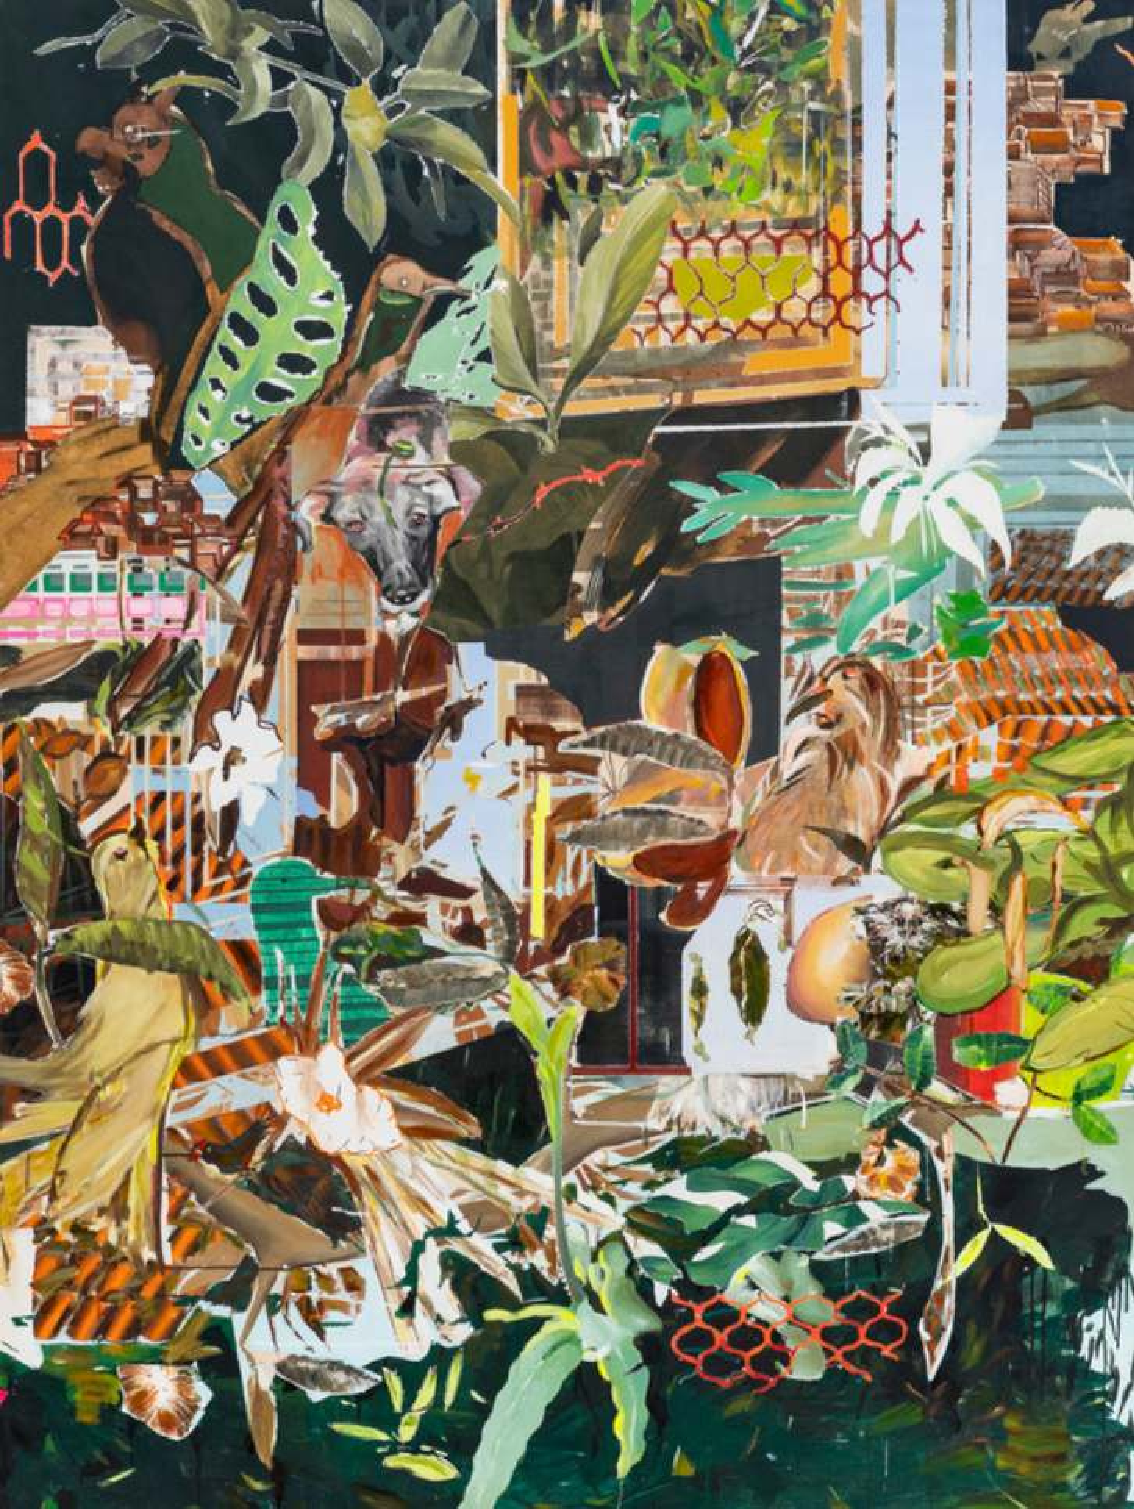
\includegraphics[width=2.38516in,height=3.3184in]{figuras/laguna-jardim53-2021.pdf.compressed.pdf}
		\figurenote{\oleo. \artsize{200x150}.}
	\end{minipage}\hfill
	\begin{minipage}{.45\linewidth}
		\caption{\artname{Lucia Laguna}{Jardim n\textordmasculine.~55}}
		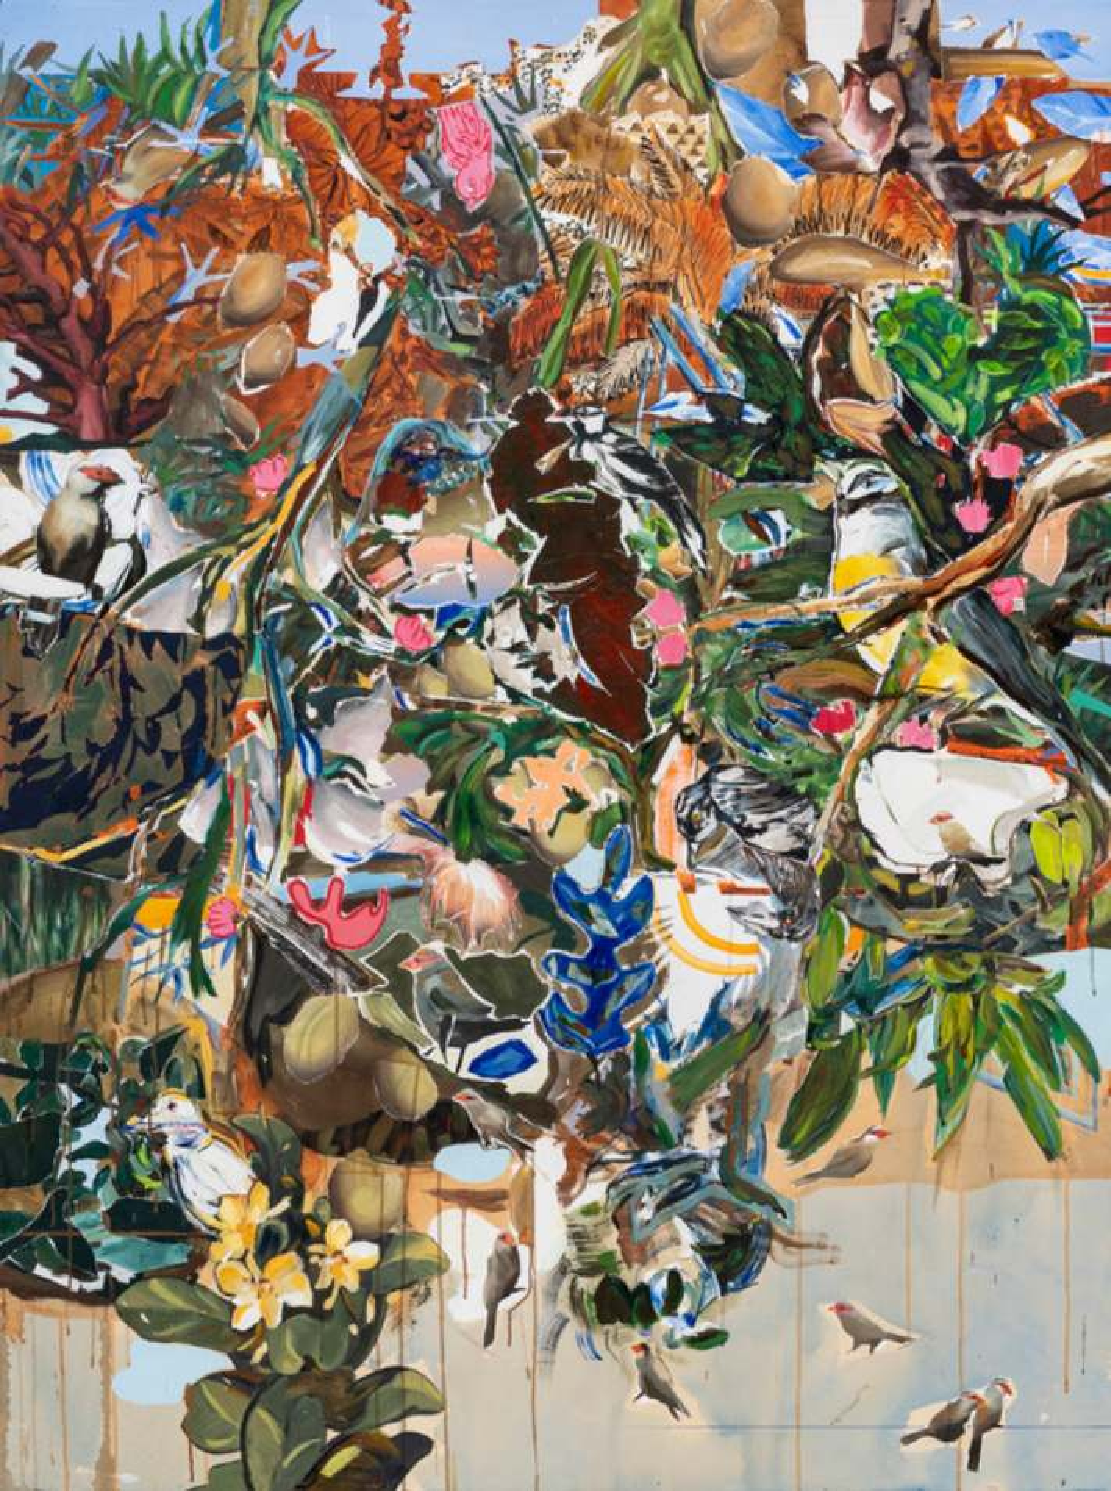
\includegraphics[height=3.3184in]{figuras/laguna-jardim55-2021.pdf.compressed.pdf}
		\figurenote{\oleo. \artsize{200x150}.}
	\end{minipage}
\end{figure}

Segundo ele, não se trata de um trabalho cujas figuras sejam o assunto
principal. Estas figuras são uma espécie de aparições, que ajudam a dar
o movimento que comenta a própria pintura. Marcelo lembra Levi Strauss,
que dizia que toda paisagem é uma imensa desordem, e identifica na
incompletude das figuras nas pinturas uma desordem calculada que remete
à paisagem. Segundo Lucia, seu processo atual é uma colagem onde ela
traz os elementos do seu jardim, como plantas, pássaros, e objetos de
uma maneira organizada e também desorganizada \parencite{gabriel2022laguna}.
Ela explica que antes de pintar qualquer imagem, faziam um recorte com
a tinta acrílica branca, e sobre este recorte era feita a pintura.



A inevitável borda fininha que sobrava, reforçava a ideia de colagem.

Diante da trajetória de Lucia Laguna, poderíamos afirmar que a paleta
tropical, característica de muitos pintores brasileiros contemporâneos,
com altos cromas, difere em muito dos trabalhos dos primeiros
colagistas dadaístas do início do século, bem como os seus assuntos,
apartados por um grande hiato temporal. No entanto, o acúmulo de
figuras no trabalho da Lúcia, além de querer representar o tema da
paisagem a que se refere Marcelo Campos, nos leva a pensar sobre o
acúmulo de imagens presentes no mundo atual, repleto de mudanças
drásticas. Este acúmulo talvez seja o mesmo que inspirou os pintores e
artistas do início do século XIX e que continuam ecoando questões de
desordem no ateliê de muitos artistas contemporâneos.

Observamos que grande parte do que escrevemos sobre o trabalho de Lucia
Laguna dizia respeito ao seu relacionamento com referências. Seja no
estudo de artistas pelos quais se interessa, seja no conceito de
acúmulo de imagens presente na história da colagem ou ainda nas
referências temáticas do seu dia a dia, cujo assunto principal é o que
vê através de sua janela ou do seu jardim. Isto me faz retomar o
assunto principal desta pesquisa, que quer construir uma imagem pintada
por meio de outro olhar, o do cinema. Podemos pensar que deixar entrar
uma imagem intermediada pela câmera, e devolvê-la ao mundo através de
um processo artístico de pintura, ou ainda se utilizar de processos
cinematográficos para realizar uma pintura é uma forma de absorver
referências. São recortes do mundo real que escolhemos para editar.
Estamos interligando olhares distintos. Visadas que pertencem não só ao
nosso mundo, mas também ao mundo do outro. Neste sentido, aquilo que
move o artista termina por se conectar, ainda que não haja uma
intencionalidade, com o olhar do outro.

\section{A intrincada trama de padrões e cores na obra de Cristina Canale}%
\label{a-intrincada-trama-de-padruxf5es-e-cores-na-obra-de-cristina-canale}

Cristina Canale iniciou seus estudos na Escola de Artes Visuais do
Parque Lage, no Rio de Janeiro, aos 18 anos de idade e em 1984
participou da histórica mostra \enquote{Como vai você, Geração 80?} Nos
anos 1990 foi estudar na Academia de Artes de Düsseldorf, na Alemanha e
fixou residência em Berlim, onde mora e trabalha atualmente. Na
entrevista para o editor de cultura e \emph{lifestyle} da Vogue,
\citeauthor{mello2021canale}, fala sobre a sua primeira individual em Nova York em 2021, na
Galeria Nara Roesler, e explica:

\begin{displaycquote}{mello2021canale}[.]
	Eu olho muita imagem do Instagram, retratos clássicos da Renascença, o
	começo dos retratos burgueses e imagens de moda, daí fui desenvolvendo
	estes retratos. Também paralelo a isso, um trabalho que já faço há 30
	anos, é trabalhar com a paisagem que comecei a pensar em colocar essa
	estética retratista de paisagem. Então eu fechei com essa série de
	retratos e a introdução é esse ambiente mais aberto de uma perspectiva
	mais ampla, que é a paisagem
\end{displaycquote}

A característica orgânica da figura humana, em forma de retrato, nem
sempre esteve tão presente em suas pinturas, como estas que tem
apresentado recentemente. Nos primeiros anos (1984--1990) o tema da
paisagem serviu de álibi para uma pintura muito matérica e onde o
embate com a tela e a tensão se travava por meio de um acúmulo grande
de tinta.

\begin{figure}[b]
	\begin{minipage}{.45\linewidth}
		\caption{\artname{Cristina Canale}{Arquipélago}{1990}}
		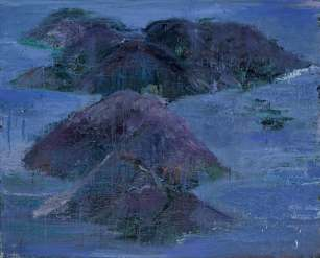
\includegraphics[width=2.42898in,height=1.95536in]{figuras/canale-arquipelago-1990.pdf.compressed.pdf}

		\figurenote{Fonte:
			\hiperlink{http://www.cristinacanale.com/obras-works-1984-1990-Arquipélago-1990}{Website de Cristina Canale}}
	\end{minipage}
	\begin{minipage}{.45\linewidth}
		\caption{\artname{Cristina Canale}{\emph{New Age}}{1991}}
		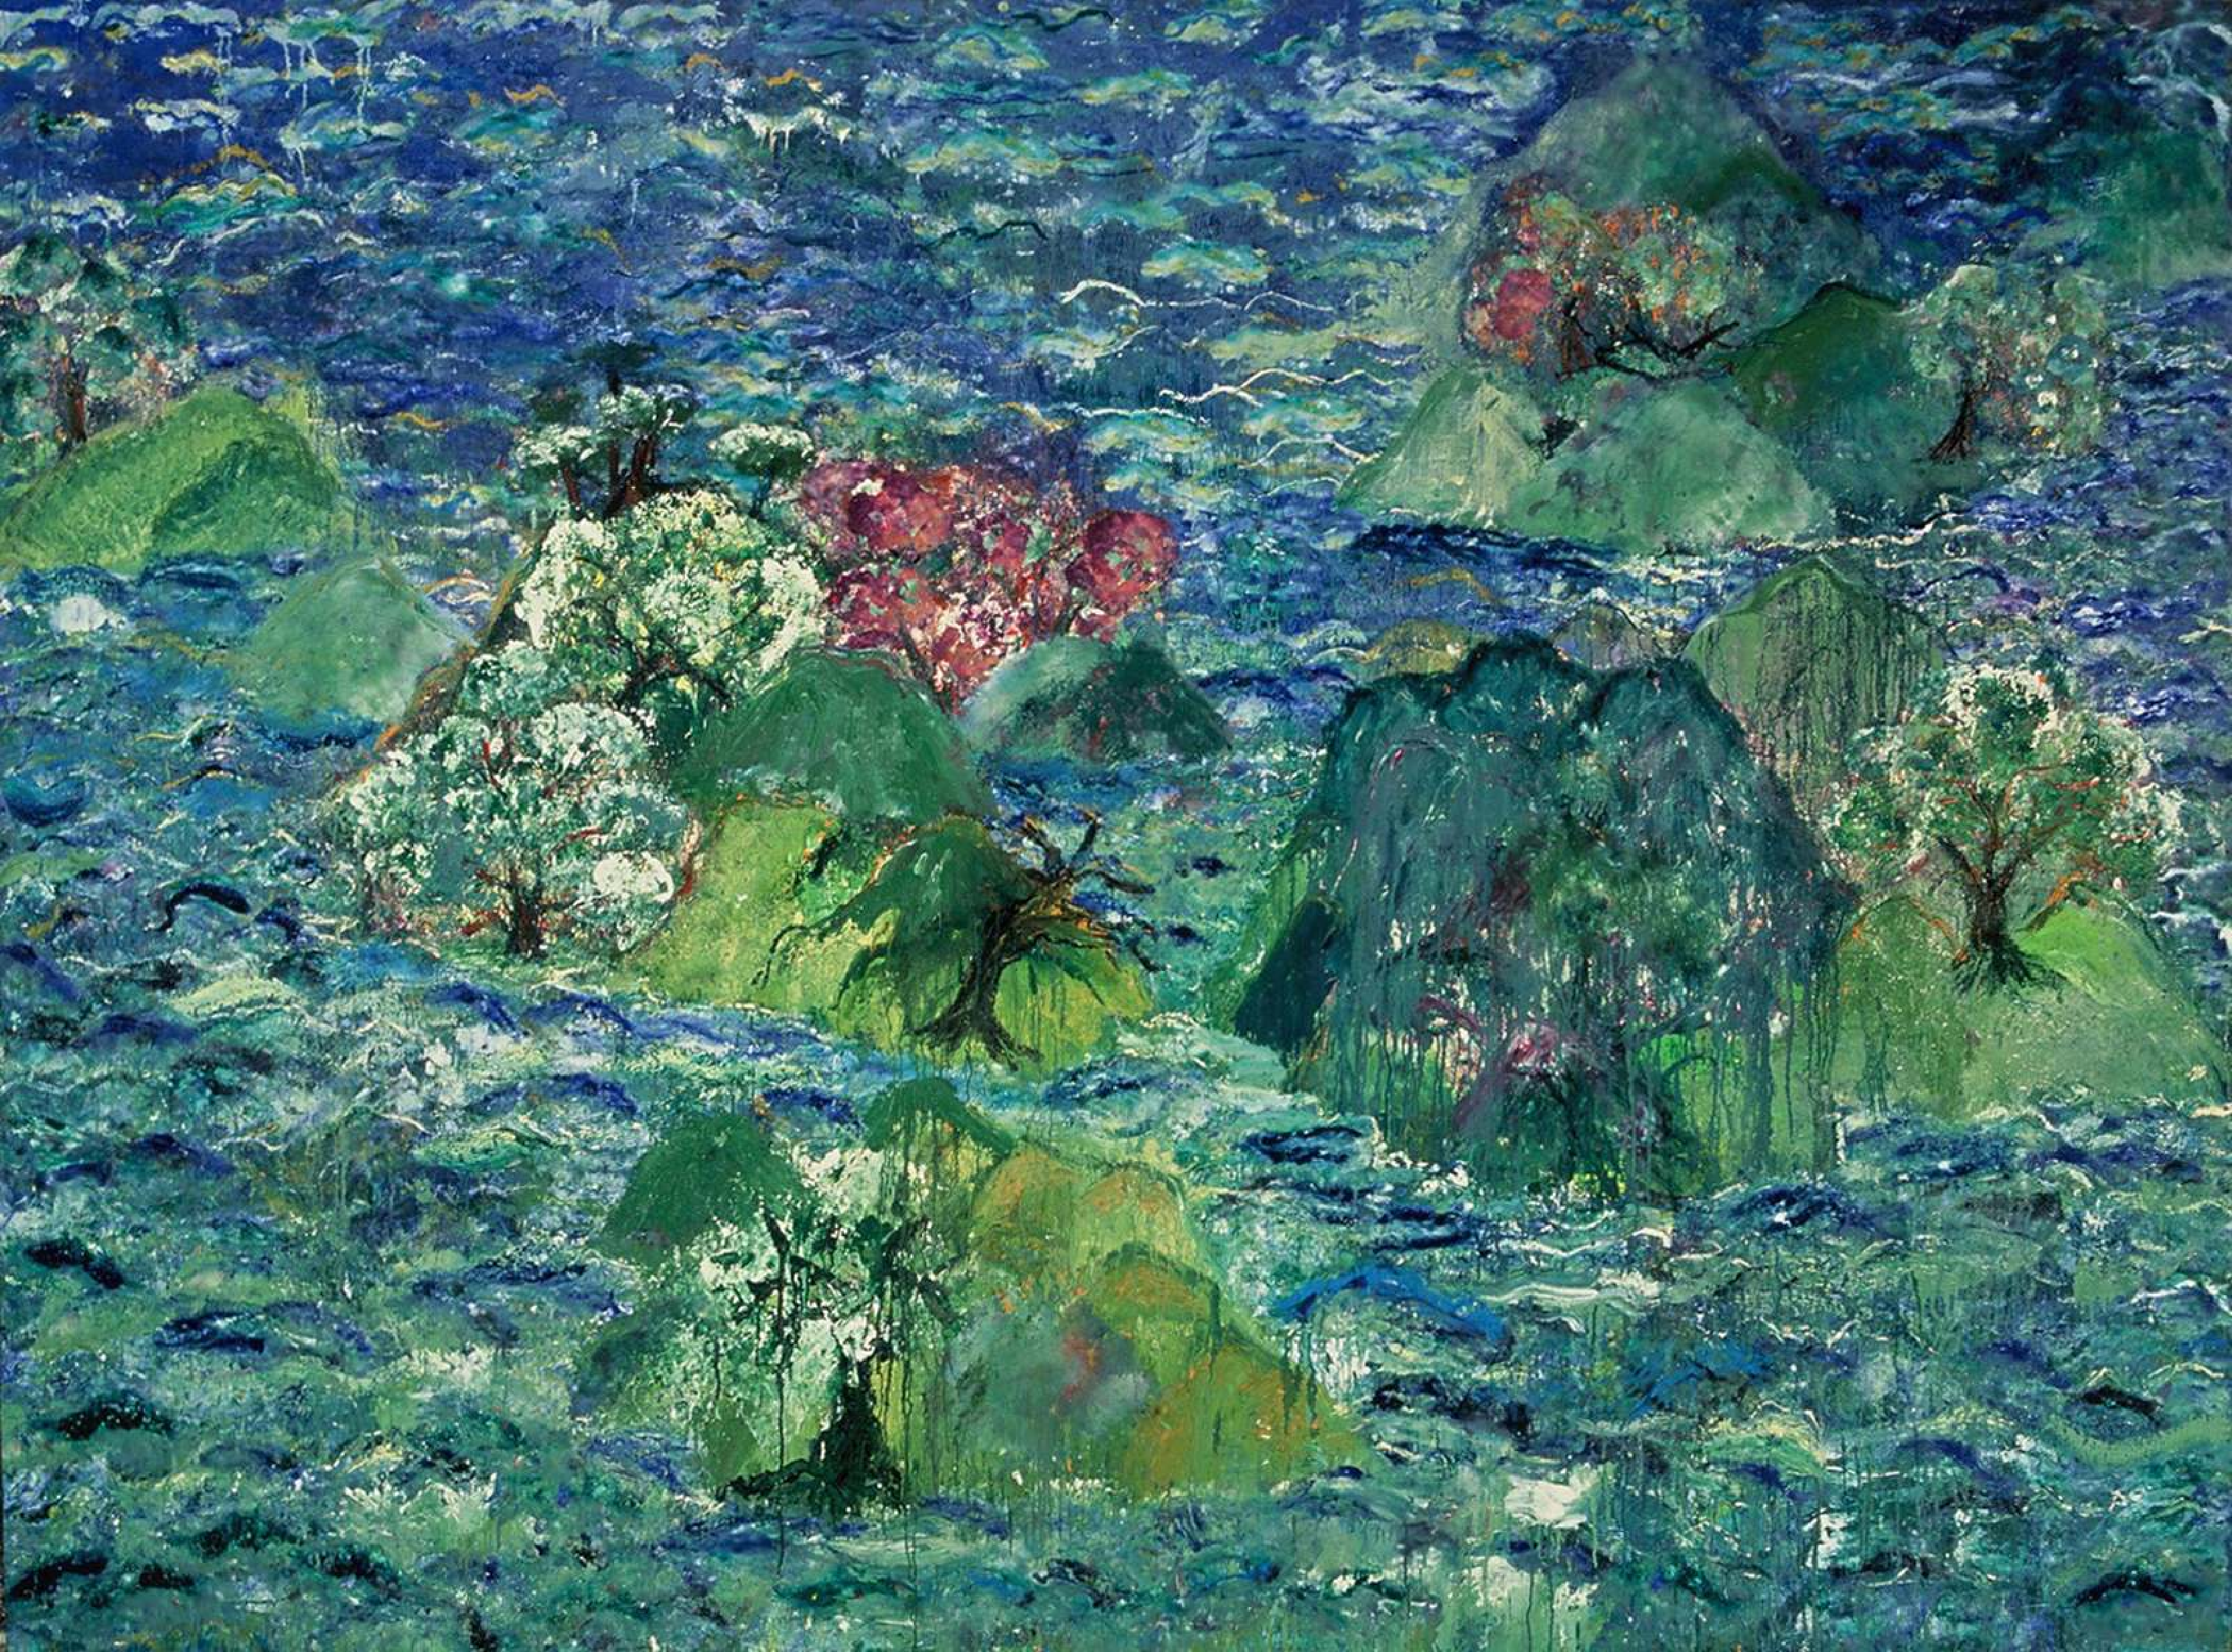
\includegraphics[width=2.6407in,height=1.95427in]{figuras/canale-new-age-1991.pdf.compressed.pdf}
		\figurenote{Fonte: \hiperlink{www.cristinacanale.com/obras-works-1991-1999-New age-1991}{Website de Cristina Canale}}
	\end{minipage}
\end{figure}
\clearpage

Analisando a trajetória de Cristina Canale, identificamos no texto
\enquote{Cristina lutadora}, de Frederico Moraes, em 1987, na exposição
realizada no Centro Empresarial Rio, na cidade do Rio de Janeiro, uma
alusão ao seu vigor gráfico em desenhos e croquis, apreendendo não só a
paisagem carioca, mas fazendo uma leitura de obras construtivistas. A
cruz de Malevitch se torna presente na pintura instalada na paisagem,
ganhando um significado perturbador, como o das pinturas de Kiefer e de
cemitérios \parencite{demoraes1987cristina}.

\begin{figure}
	\caption{\artname{Cristina Canale}{Os Sobreviventes}{1990}}
	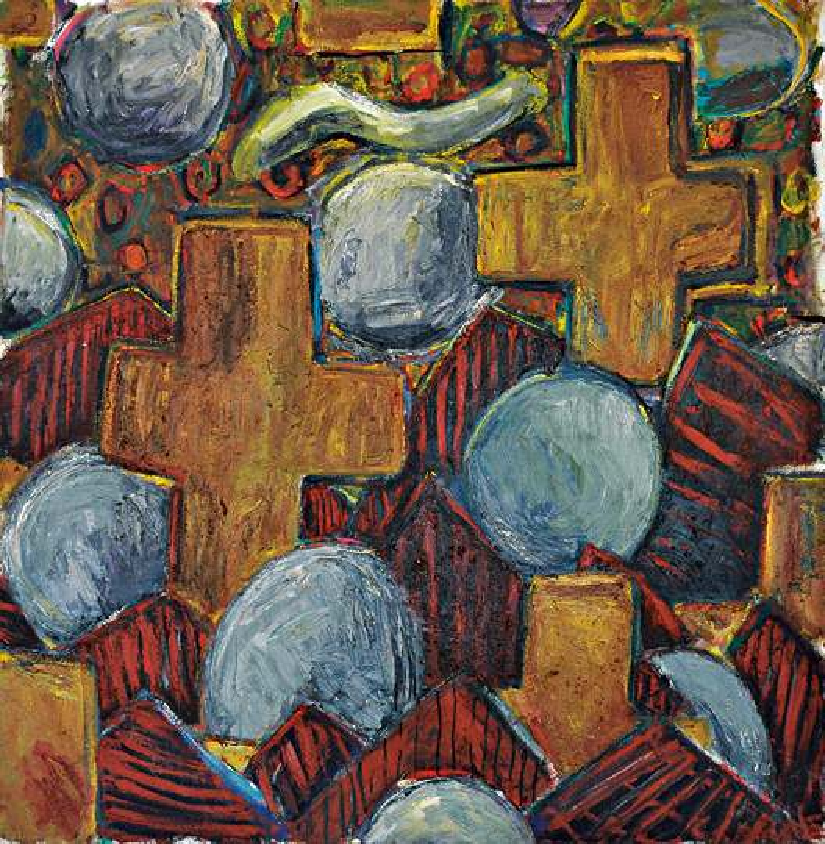
\includegraphics[width=2.22414in,height=2.27465in]{figuras/canale-sobreviventes-1985.pdf.compressed.pdf}

	\figurenote{Fonte: \hiperlink{www.cristinacanale.com/obras-works-1984-1990-Os sobreviventes-1985}{Website de Cristina Canale}}
\end{figure}

Na entrevista ao crítico e curador \textcite{cocchiarale2011entre}, Cristina reforça
a alternância e a importância das referências no seu processo criativo
ao longo de sua trajetória

\begin{displaycquote}{cocchiarale2011entre}[.]
	A partir de 1985, parei com papel e parti para as telas, depois de breve
	tentativa com tinta acrílica, me dediquei à pintura a óleo sobre tela. A
	temática menos figurativa, suprimiu a figura humana de meus trabalhos
	por uns tempos. Usava as formas arquitetônicas da cidade, arcos da lapa,
	catedral, viadutos etc. Como imagens iniciais e, em seguida, procurava
	as formas arquetípicas delas, até chegar às cruzes e círculos, que
	durante um pequeno período usei para constituir paisagens (meio duras,
	lembravam mais cemitérios ou restos de uma Guerra). Este geometrismo
	durou cerca de um ano e pouco. Foi sendo suavizado e cheguei às
	paisagens mais liquidas: as cruzes viraram ilhas, por exemplo, e os
	círculos, ondas do mar. Era um mundo com muita água, mar, rios, lagoas,
	cercada de montanhas e ilhas, muita \emph{National Geographic Magazine},
	fundos de pinturas renascentistas e Rio de janeiro, claro. Quando
	cheguei à paisagem, respirei mais livremente, pude soltar cor e matéria
\end{displaycquote}

Percebemos que a figura feminina foi entrando em seu trabalho, no
período de 2010 a 2019, através de elementos vinculados à moda como
padronagens, sapatos, bolsas, e vestes que aos poucos perderam seu
protagonismo para figuras inteiras em ambientes cotidianos. Quando em
entrevista para a \url{Vogue.com} é questionada sobre como o interesse por
moda se manifesta em seu trabalho, Cristina alega não saber o que veio
primeiro, o ovo ou a galinha:

\begin{displaycquote}{mello2021canale}[.]
	Acho que desde garota eu me interesso por moda para comprar e sair
	usando, isso é outro ponto. E eu me interesso por formas, eu gosto de
	ler sobre a história das formas,~mas leio assim, superficialmente.
	Também não chego a ser uma socióloga da moda, mas~compro uns livros
	para ver a história das roupas, como começou, mas acho que é um
	interesse muito particular. Muitas das soluções de moda vieram de
	uniformes militares que foram sendo usados civilmente, ou como as
	mulheres começaram a solucionar de onde vinha, ou, mais contemporâneo,
	como algumas soluções de moda vieram de esporte, de hipismo\ldots\ são
	várias informações que eu gosto de ir colocando. Muitas roupas quase
	são esculturas às vezes. Isso me interessa
\end{displaycquote}

\begin{figure}
	\begin{minipage}[t]{.45\linewidth}
		\caption{\artname{Cristina Canale}{Desfile}{2012}}
		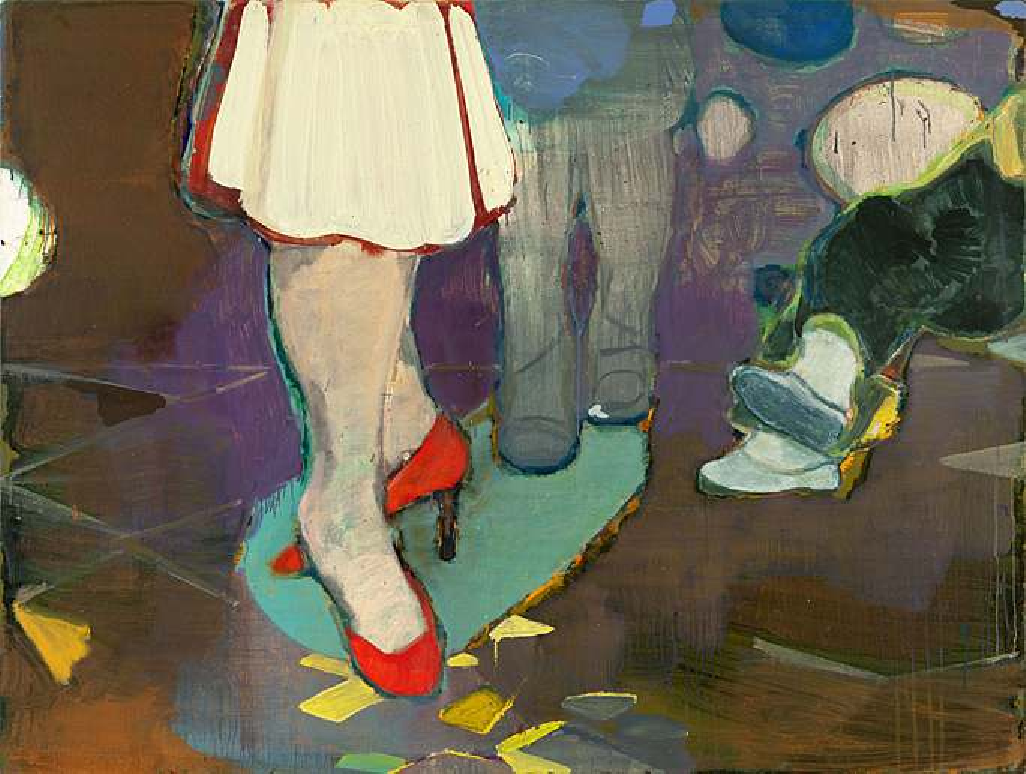
\includegraphics[height=1.95in]{figuras/canale-desfile-2012.pdf.compressed.pdf}
		\figurenote{Fonte: \hiperlink{cristinacanale.com/obras-works-2010-2019-Desfile-2012}{Website de Cristina Canale}.}
	\end{minipage}\hfill
	\begin{minipage}[t]{.45\linewidth}
		\caption{\artname{Cristina Canale}{Mimetismo}{2012}}
		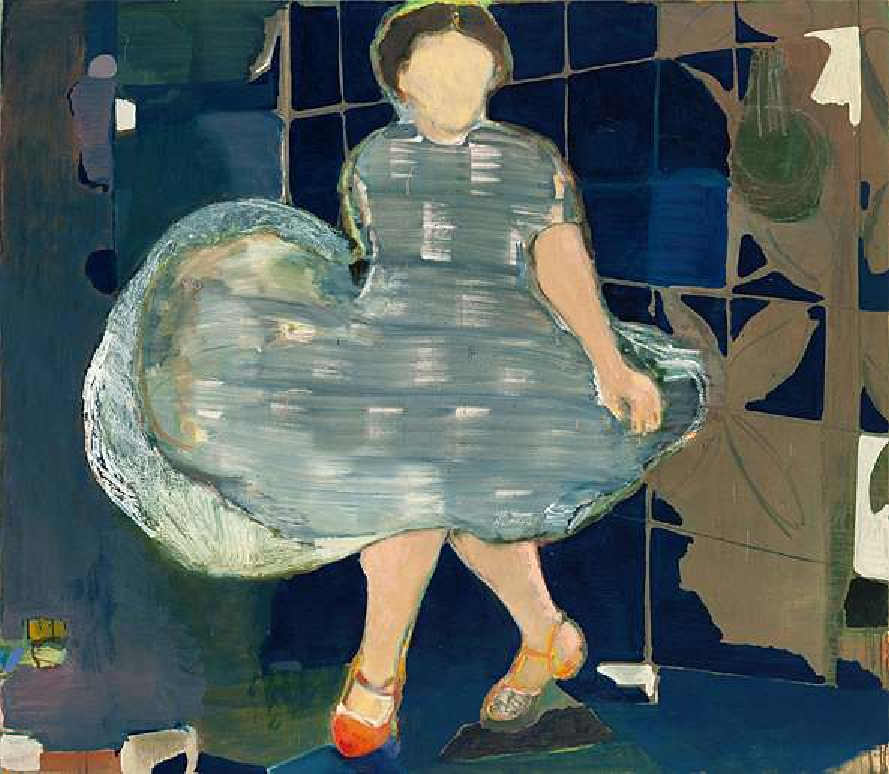
\includegraphics[height=1.95in]{figuras/canale-mimetismo-2012.pdf.compressed.pdf}
		\figurenote{Fonte: \hiperlink{cristinacanale.com/obras-works-2010-2019-Mimetismo-2012}{Website de Cristina Canale}}
	\end{minipage}
\end{figure}

\begin{figure}
	\begin{minipage}{.45\linewidth}
		\caption{\artname{Cristina Canale}{Geoportátil}{2016}}
		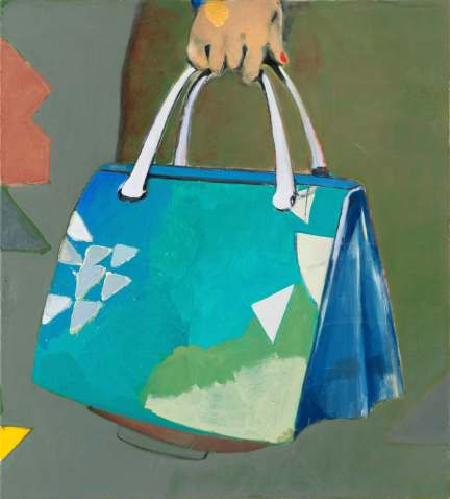
\includegraphics[height=2in]{figuras/canale-geoportatil-2016.pdf.compressed.pdf}
		\figurenote{\hiperlink{cristinacanale.com/obras-works-2010-2019-Geoportatil-2016}{Website de Cristina Canale}}
	\end{minipage}\hfill
	\begin{minipage}{.45\linewidth}
		\caption{\artname{Cristina Canale}{Submarino}{2012}}
		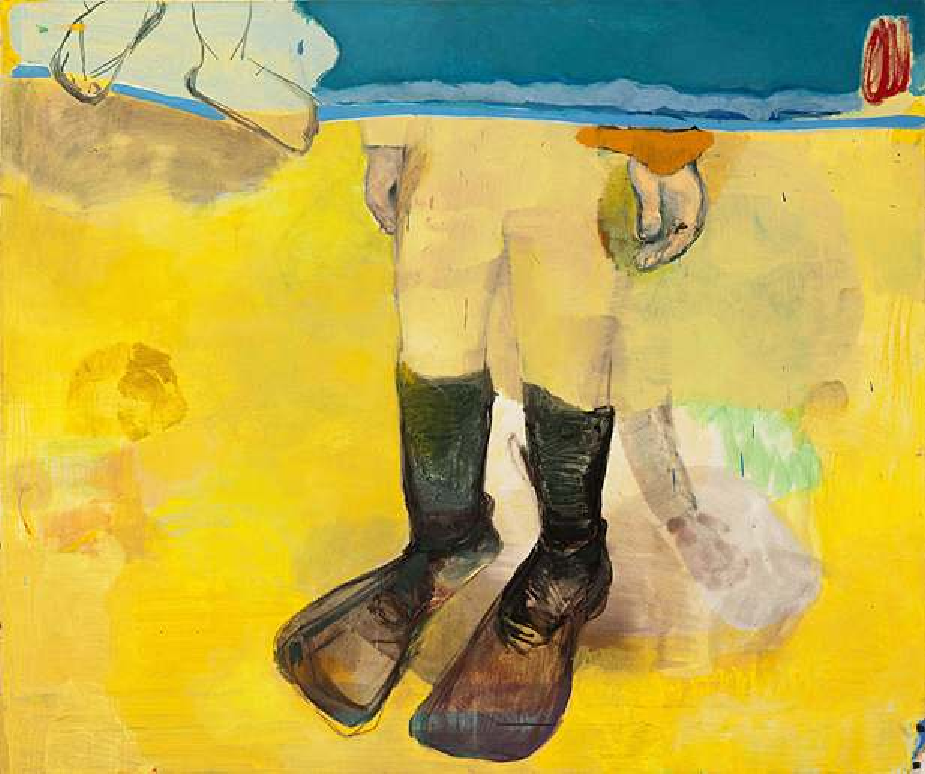
\includegraphics[height=2in]{figuras/canale-submarino-2012.pdf.compressed.pdf}
		\figurenote{\hiperlink{www.cristinacanale.com/obras-works-2010-2019-Submarino-2012}{Website de Cristina Canale}}
	\end{minipage}
\end{figure}

A padronagem herdada da moda, no trabalho de Cristina, assume uma
função importante dentro da negociação entre o abstrato e o figurativo.
Um ponto chave de toda sua produção é tensionar a convivência entre
contraditórios. A cor entra naturalmente em seu trabalho, mas não menos
importante, do que forma. O texto da curadora \textcite{diniz2018cabecas} ressalta
este papel decisivo da cor:

\begin{displaycquote}{diniz2018cabecas}[.]
	Em suas pinturas, é sobretudo por meio da cor que essas intensidades vão
	se configurando e negociam espaço, densidade e movimento entre si. Na
	produção da artista, desde cedo é a cor (e não o traço ou os planos) que
	tem \enquote{força dimensional}, fundando arranjos pictóricos que organizam
	níveis no espaço sem que, todavia, esses se comportem de acordo com a
	exatidão planar da tradição euclidiana. Por organizar e hierarquizar a
	espacialidade da pintura, como sublinha Canale, a \enquote{cor é funcional}.
	Preponderantemente, contudo, ela é intensiva, fazendo \enquote{vibrar} as
	coisas em seus lugares e estados, animando o que poderia parecer estável
	se não fosse continuamente inquietado por uma espécie de viço que emana
	das cores
\end{displaycquote}

Se observamos em Lucia Laguna referências relacionadas a outros
pintores e a espaços reais como os que vê através da janela de seu
ateliê e do seu jardim, na obra de Cristina Canale, percebemos uma
motivação pessoal, com cenas do cotidiano que partem de imagens de
revistas de moda e redes sociais como fonte de pesquisa.
